\documentclass[12pt,a4paper,titlepage,headinclude,bibtotoc]{scrartcl}

%---- Allgemeine Layout Einstellungen ------------------------------------------

% Für Kopf und Fußzeilen, siehe auch KOMA-Skript Doku
\usepackage[komastyle]{scrpage2}
\pagestyle{plain}
\setheadsepline{0.5pt}[\color{black}]
\automark[section]{chapter}


%Einstellungen für Figuren- und Tabellenbeschriftungen
\setkomafont{captionlabel}{\sffamily\bfseries}
\setcapindent{0em}


%---- Weitere Pakete -----------------------------------------------------------
% Die Pakete sind alle in der TeX Live Distribution enthalten. Wichtige Adressen
% www.ctan.org, www.dante.de

% Sprachunterstützung
\usepackage[ngerman]{babel}

% Benutzung von Umlauten direkt im Text
% entweder "latin1" oder "utf8"
\usepackage[utf8]{inputenc}

% Pakete mit Mathesymbolen und zur Beseitigung von Schwächen der Mathe-Umgebung
\usepackage{latexsym,exscale,stmaryrd,amssymb,amsmath}


\usepackage[nointegrals]{wasysym}
\usepackage{eurosym}

% Anderes Literaturverzeichnisformat
%\usepackage[square,sort&compress]{natbib}
\usepackage{hyperref}
% Für Farbe
\usepackage{color}
\usepackage{graphicx}
\usepackage{wrapfig}
\usepackage{subfigure}

% Caption neben Abbildung
\usepackage{sidecap}

% Befehl für "Entspricht"-Zeichen
\newcommand{\corresponds}{\ensuremath{\mathrel{\widehat{=}}}}
% Befehl für Errorfunction
\newcommand{\erf}[1]{\text{ erf}\ensuremath{\left( #1 \right)}}

%Fußnoten zwingend auf diese Seite setzen
\interfootnotelinepenalty=1000

%Für chemische Formeln (von www.dante.de)
%% Anpassung an LaTeX(2e) von Bernd Raichle
\makeatletter
\DeclareRobustCommand{\chemical}[1]{%
  {\(\m@th
   \edef\resetfontdimens{\noexpand\)%
       \fontdimen16\textfont2=\the\fontdimen16\textfont2
       \fontdimen17\textfont2=\the\fontdimen17\textfont2\relax}%
   \fontdimen16\textfont2=2.7pt \fontdimen17\textfont2=2.7pt
   \mathrm{#1}%
   \resetfontdimens}}
\makeatother

%Honecker-Kasten mit $$\shadowbox{$xxxx$}$$
\usepackage{fancybox}

%SI-Package
\usepackage{siunitx}

%keine Einrückung, wenn Latex doppelte Leerzeile
\parindent0pt

%Bibliography \bibliography{literatur} und \cite{gerthsen}
%\usepackage{cite}
\usepackage{babelbib}
\selectbiblanguage{ngerman}

\begin{document}

\begin{titlepage}
\centering
%\textsc{\Large Praktikum zur Einführung in die physikalische Chemie,\\[1.5ex] Universität Göttingen}

\vspace*{1cm}

\rule{\textwidth}{1pt}\\[0.5cm]
{\huge \bfseries
  V1: Bestimmung\\[1.5ex]
  der Loschmidt-Zahl}\\[0.5cm]
\rule{\textwidth}{1pt}

\vspace*{3cm}


\begin{Large}
\begin{tabular}{ll}
Durchführende: &  Alea Tokita, Julia Stachowiak\\
Assistentin: & Annemarie Kehl\\
 Versuchsdatum: & 23.11.2015\\
 Datum der Abgabe: & 30.12.2015\\
\end{tabular}
\end{Large}

\vspace*{1cm}

\begin{Large}
\fbox{
  \begin{minipage}[t][8cm][t]{11cm} 
  \textbf{Werte:}\\
  \\
   Aluminium-Kristall\\
 \quad $ L_A= (7,19 \ \cdot 10^{23}  \pm 2\cdot10^{21}) \quad \ \mathrm{mol^{-1}} $\\
   \\
 Lithiumfluoridkristall\\
\quad $ L_A = (6,36 \ \cdot 10^{23} \pm 8 \cdot 10^{21}) \quad \mathrm{mol^{-1}} $\\
 \\
 Calciumchloridkristall\\
 \quad $L_A = (5,985 \ \cdot 10^{23} \pm 6 \cdot 10^{20}) \quad \mathrm{mol^{-1}}$\\
 \\
  \end{minipage}
}
\end{Large}

\end{titlepage}

\tableofcontents

\newpage

\section{Theoretische Grundlagen}
\subsection{Stoffmenge}
Im Umgang mit chemischen Reaktionen müssen Stoffmengen betrachtet werden. Da jedoch die Teilchen, mit denen sich auseinandergesetzt wird, so klein sind, ist es höchst unpraktisch mit der jeweiligen Teilchenanzahl zu rechnen. Daher wurde die Einheit Mol eingeführt, um die Stoffmenge anzugeben. Diese Einheit ist so definiert, dass $ \mathrm{1 mol}$ einer beliebigen Substanz dieselbe Anzahl von Teilchen (Moleküle, Atome, Ionen) enthält, wie Atome in $\mathrm{12g}$ des Kohlenstoff-Isotops $\mathrm{^{12}C}$ enthalten sind. Diese Zahl an Teilchen, die in einem Mol enthalten sind, wird durch die Loschmidt-Zahl $N_{A}$ (oder auch Avogadro-Konstante oder Avogadro-Zahl) angegeben:\\

\begin{center}
$N_{A}=6,02214129(27)\cdot 10^{23}\ \mathrm{mol^{-1}}$ 
\end{center}

Mit dieser Zahl lässt sich nun die Molmasse \textit{M} einer Substanz angeben, welche die Masse eines Mols einer Sunstanz in der Einheit $ \mathrm{g \cdot mol^{-1}}$ bezeichnet. Analog bezeichnet das Molvolumen $V_{m}$ das Volumen, welches von einem Mol eines Stoffes eingenommen wird. Dieses Volumen ist temperatur- und druckabhängig.

\subsection{Elementarzelle}
In einem Kristall sind Teilchen (Atome, Ionen, Moleküle) in symmetrischer und geordneter Weise in einem sich periodisch wiederholenden, dreidimensionalen Muster angeordnet. Diese Symmetrie eines Kristalls kann mithilfe eines Kristallgitters beschrieben werden. Indem die Mittelpunkte der Teilchen gedanklich durch Gitterpunkte ersetzt werden, lässt sich aus einer Kristallstruktur ein Kristallgitter ableiten.\\

Ein Kristallgitter kann in lauter identische Elementarzellen zerlegt werden. Das Gitter ist also aus wiederholt in alle Raumrichtungen aneinandergereihte Elementarzellen aufgebaut. Dies lässt sich wieder auf die Kristallstruktur übertragen: Da der Kristall durch wiederholtes aneinanderlegen der Elementarzellen aufgebaut ist, muss die chemische Zusammensetzung einer Elementarzelle exakt der Zusammensetzung der Substanz entsprechen\footnote{Vgl. Mortimer s. 180}.\\\\

Je nach ihrer Symmetrie können Kristallgitter in Gittertypen eingeteilt werden, die sich in der Metrik ihrer Elementarzellen unterscheiden\footnote{Vgl. Mortimer}. Mithilfe von Röntgenstrahlung bekannter Wellenlänge kann die Strukur und Größe einer Elementarzelle, also ihre Gitterstruktur und Gitterkonstante \textit{a} bestimmt werden. Hier eine Darstellung dieser Größe an den von uns vermessenen Kristallen:




\begin{figure} [h]
\begin{center}
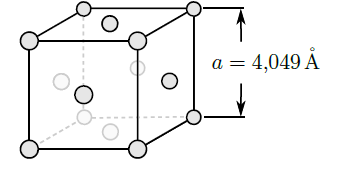
\includegraphics[scale=0.7]{Aluminium.png} \end{center}
\caption{Kristallstruktur von Aluminium$^a$}
\end{figure}

\begin{figure} [h]
\begin{center}
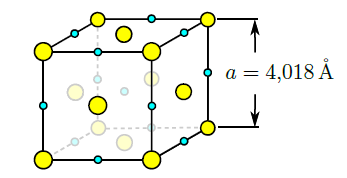
\includegraphics[scale=0.7]{Lithiumflourid.png} \end{center}
\caption{Kristallstruktur von Lithiumflourid$^b$}
\end{figure}

\begin{figure} [h]
\begin{center}
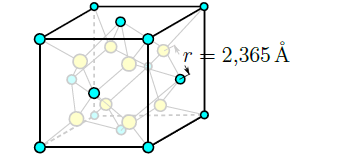
\includegraphics[scale=0.7]{Calciumflourid.png} \end{center}
\caption{Kristallstruktur von Kalziumflourid$^c$}
\end{figure}

\hrulefill\\
$^{a,b,c}$ Skriptum für das Praktikum zur Einführung in die Physikalische Chemie, Seite 2.

\vspace{10cm}
In den Bespielen liegt bei den ersten beiden Kristallen ein kubisch-flächenzentriertes Gitter und bei dem letzen Kristall ein kubisch-flächenzentriertes Gitter aus $\mathrm {Ca^{2+}-Ionen}$ und ein kubisch-primitives Gitter aus $ \mathrm {F^{-}-Ionen vor}$. Des weiteren gibt es etwa tetragonale, hexagonale, rhomboedrische sowie viele weitere Strukturen.\\ Eine primitive Elementarzelle enthält von jeder Atomart nur ein äquivalentes Atom. Die acht Atome in den Eckpunkten der Elementarzellen gehören nur zu einem achtel zu der Elementarzelle, da an jeder Ecke acht Elementarzellen aufeinander treffen.\\
In einer flächenzentrierten Elementarzelle befinden sich in den Ecken und in den Mitten aller sechs Flächen äquivalente Atome. Ein Atom auf einer Fläche gehört der Zelle zur Hälfte, eines auf der Kante zu einem viertel und eines im Zentrum der Zelle ganz.\\
Mithilfe dieser Informationen lässt sich berechnen, wie viele Formeleinheiten $N_{Z}$ auf eine Elementarzelle kommen. Beispielsweise kommt auf eine primitive Elementarzelle eine Formeleinheit, da wir acht Teilchen haben, die der Elementarzelle zu je einem achtel gehören.\\\\ Mithilfe folgender Überlegungen lässt sich die Masse $m_{Z}$ einer Elementarzelle bestimmen:

\begin{equation}
m_{Z}=Nz \cdot \dfrac{M}{N_{A}}
\end{equation} 

Das Volumen der Elementarzellen unserer zu untersuchender Kristalle lässt sich wie das Volumen eines Würfels folgendermaßen berechnen.

\begin{equation}
V_Z = a^3
\end{equation}


\subsection{Bestimmung der Loschmidt-Zahl}
 
Ziel des Versuchs ist es, die Loschmidt-Zahl $N_{A}$ durch den Vergleich von makroskopischer Dichte $p_{makro}$ mit mikroskopischer Dichte $p_{mikro}$ von exakt geformten, zylindrischen Lithiumflourid-, Calciumflourid- und Aluminiumkristallen, zu bestimmen.\\\\

Die Makroskopische Dichte lässt sich durch  Masse und Volumen der Probekörper wie folgt errechnen:

\begin{equation}
p_{makro}= \frac{m_{Zyl}}{V_{Zyl}}
\end{equation}

Das Volumen des zylindrischen Probekörpers kann dabei durch genaue Bestimmung von Radius $r$ und Länge $l$ mithilfe folgender Formel bestimmt werden:

\begin{equation}
V_{zyl} = \pi \cdot r^{2} \cdot l
\end{equation}

Für die mikrospische Dichte $p_{mikro}$ einer Elementarzelle gilt, dass sie identisch zu der Makroskopischen Dichte ist, da ein Kristall durch die periodische Wiederholung seiner Elementarzellen aufgebaut ist.

\begin{equation}
p_{mikro}=\frac{m_Z}{V_Z}
\end{equation}

Masse und Volumen der Elementarzelle lassen sich mithilfe der oben aufgeführten Gleichungen 1 und 2 berechnen. Somit gilt unter Annahme, dass die makroskopische Dichte identisch zur mikroskopischen ist:

\begin{equation}
\frac{m_{Zyl}}{V_{Zyl}}= \frac{Nz \cdot M}{N_{A} \cdot a^3}
\end{equation}

Dies lässt sich nun nach $N_A$ umformen und ergibt folgende Formel zur Berechnung der Loschmidt-Zahl:

\begin{equation}
N_A= \frac{N_Z \cdot M \cdot V_{Zyl}}{a^3 \cdot m_{Zyl}}
\end{equation}

\subsection{Bestimmung von $a$ des Kalciumflouridkristalls}
 
Um die Loschmidt-Zahl zu bestimmen wird der Wert $a$, die Kantenlänge einer Elementarzelle, benötigt. Dieser ist für die meisten Kristalle schon gegeben, lediglich für den Kalziumchlorid-Kristall muss sie noch ermittelt werden. Abbildung 3 zeigt die Kristallstruktur von Kalziumflourid. Es ist ein größeres kubisch-flächenzentriertes Gitter von $ \mathrm {Ca^{2+}}$-Ionen sowie ein darin liegendes, kleineres kubisch-primitives Gitter von $ \mathrm{F^-}$-Ionen erkennbar. Als Information ist uns der Abstand $r$ von den Ionen gegeben. Bei genauerer Betrachtung des Kristalls ist zu erkennen, dass ein Fluorid-Ion tetraedrisch von je vier Kalzium-Ionen umgeben ist. Der Abstand vom Zentrum zu den Ecken des Tetraeders entspricht dabei dem Abstand $r$.

\begin{figure} [h]
\begin{center}
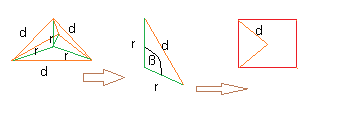
\includegraphics[scale=1]{a.png} \end{center}
\caption{Berechnung von $a$}
\end{figure} 

\newpage

So lässt sich nun die Länge $d$ mithilfe des Kosinussatzes berechnen, da der Winkel in einem Tetraeder allgemein mit $109,5^\circ$ bekannt ist:

\begin{equation}
 d = \sqrt{2r^2-2r^2 \cdot \cos \beta } = 3, 863 \quad \AA
\end{equation}     

Die Länge $d$ ist die Hälfte der Flächen-diagonalen des Kalzium-Ionengitters. Da der Winkel zwischen den Flächen-diagonalen allgemein mit $ 90^\circ $ bekannt ist, lässt sich wieder mithilfe des Kosinussatzes die Länge $a$ berechnen:

\begin{equation}
 d = \sqrt{2d^2-2d^2 \cdot \cos \gamma } = 5,463 \quad \AA
\end{equation}   

\section{Experimentelles}


\subsection{Versuchsaufbau}
\begin{figure} [h]
\begin{center}
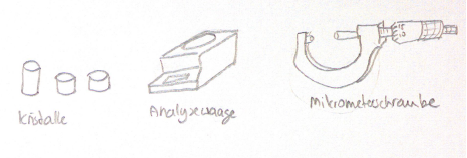
\includegraphics[scale=1]{Versuchsaufbau2.png} \end{center}
\caption{Versuchsaufbau}
\end{figure} 

\subsection{Hilfsmittel}
Als Hilfsmittel werden eine Analysewaage sowie eine Mikrometerschraube verwendet.

\subsection{Durchführung}

Für die Bestimmung der Loschmidt-Zahl werden die drei Kristalle jeweils zehnmal gewogen und ausgemessen. Mithilfe der Analysewaage wird die Masse $m_{Zyl}$ bestimmt. Mit der Mikrometerschraube wird die Länge $l$ und Durchmesser $d$ gemessen. Im Umgang mit den Kristallen müssen Baumwollhandschuhe getragen werden. 

\newpage
\section{Auswertung}
Zur Bestimmung der Loschmidt -Zahl wird nach der in Kapitel 1.3 beschriebenen Vorhergehensweise vorgegangen. Zuerst muss der Mittelwert der verschiedenen Messgrößen errechnet werden:
\begin{equation}
\bar{x}=\frac{1}{N} \sum_{i=1}^N x_i
\end{equation}

Für die gemessenen Werte ergeben sich somit folgende Mittelwerte:\\

\vspace{3mm}
\textbf{Aluminiumkristall:}\\
Masse $\bar{m}=9,9446$ \ g \\
Durchmesser $\bar{d}=15,00$ \ mm \\
Länge $\bar{l}=24,88$ \ mm\\

\vspace{3mm}
\textbf{Lithiumfluorid-Kristall:}\\
Masse $\bar{m}=15,8498$ \ g \\
Durchmesser $\bar{d}=25,88$ \ mm \\
Länge $\bar{l}=11,96$ \ mm\\

\vspace{3mm}
\textbf{Calciumfluorid-Kristall:}\\
Masse $\bar{m}=10,0479$ \ g \\
Durchmesser $\bar{d}=19,98$ \ mm \\
Länge $\bar{l}=10,00$ \ mm\\

Mit $r=\frac{d}{2}$ lassen sich mithilfe von Formel 4 folgende Volumina berechnen:

\vspace{3mm}
$V_{Aluminiumkristall} = 6299 \quad \mathrm{mm^3}$\\
$V_{Lithiumfluorid-Kristall} =4398 \quad \mathrm{mm^3}$\\
$V_{Calciumfluoridkristall} = 3138 \quad \mathrm{mm^3}$\\

\vspace{3mm}

Daraus ergeben sich für die Loschmidt-Zahl nach Formel 7 folgende Werte:
\vspace{3mm}

Aluminium-Kristall: \qquad $N_A = 7,190 \ \cdot 10^{23} \quad \mathrm{mol^-1}$\\
mit $N_Z =4$ und $a=4,049\cdot 10^{-7} $ mm\\
\vspace{3mm}

Lithiumfluoridkristall: \qquad $N_A = 6,360 \ \cdot 10^{23} \quad\mathrm{mol^-1}$\\
mit $N_Z =4$ und $a=4,018\cdot 10^{-7} $ mm\\
\vspace{3mm}

Calciumchloridkristall: \qquad $N_A = 5,985 \ \cdot 10^{23} \quad\mathrm{mol^-1}$\\
mit $N_Z =4$ und $a=5,4627\cdot 10^{-7} $ mm\\
\vspace{3mm}


\section{Fehlerrechnung}
Fehler bei dem Versuch entstehen für jede der drei Messungen an dem Kristall. Der Fehler, bzw. die Messungenauigkeit der verwendeten Geräte muss berücksichtigt werden. Ein andere Fehlergröße ist die Standartabweichung des Mittelwertes, die den statistischen Fehler des Mittelwertes angibt. 
Diese beiden Fehler müssen für jede der drei Messgrößen berücksichtigt werden.

Die Gerätefehler bzw. -ungenauigkeiten sind für alle Messungen gleich und ergben sich aus der ersten vom Gerät nicht genau definierten Dezimalstelle:
\\
\\
$\Delta m = 0,00005$ g \\
$\Delta d = 0,005$ mm\\
$\Delta l = 0,005 $ mm\\
\\

Die Standartabweichung des Mittelwertes muss für jede Messung einzeln ausgerechnet werden. Sie ergibt sich durch folgende Formel:

\begin{equation}
\bar{s_N}=\sqrt{\frac{1}{N-1}\sum_{i=1}^N (x_i -\bar{x})^2}
\end{equation}

Diese entstandenen Fehler setzen sich im Laufe der Rechnung fort und müssen bei der Berechung von $N_A$ mit berücksichtigt werden. Dafür wird das Gauß'sche Fehlerfortpflanzungsgesetz angewandt:

\begin{equation}
\Delta f =\sqrt{\sum_{i} \left( \frac{\delta f}{\delta x_i}\right)^2 \cdot\Delta x^2_i }
\end{equation}

Somit ergibt sich folgender Fehler für $N_A$:

\begin{equation}
\Delta f = \sqrt{\left(\frac{N_z \cdot M \cdot \pi \cdot 2d \cdot l}{m_{Zyl} \cdot a^3 \cdot 4}\right)^2 \cdot \Delta d^2 + \left(\frac{N_z \cdot M \cdot \pi \cdot d^2 \cdot 1}{m_{Zyl} \cdot a^3 \cdot 4}\right)^2 \cdot \Delta l^2 - \left(\frac{N_z \cdot M \cdot \pi \cdot d^2 \cdot l}{m_{Zyl}^2 \cdot a^3 \cdot 4}\right)^2 \cdot \Delta m^2}
\end{equation}

\subsection{Aluminiumkristall}
 
Mithilfe der Standartabweichung des Mittelwertes wurden folgende Fehler für die einzelnen Größen berechnet:
\\
\\
$\Delta m = 5,2068\cdot10^{-5} \ \mathrm{g} \quad \Delta d= 00,01659 \ \mathrm{mm} \quad \Delta l = 0,01059\ \mathrm{mm}$\\

\vspace{3mm}
Bei Vergleich der Gerätefehler wird deutlich, dass sich beide Fehler in ungefähr derselben Größenordnung befinden und somit keiner der beiden Fehler überwiegt und der andere vernachlässigt werden kann. Somit müssen die beiden Fehler für die verschiedenen Größen addiert werden und es ergeben sich folgende Werte:

\vspace{3mm} 
$\Delta m =5,5207\cdot 10^{-4}\ \mathrm{g} \qquad\Delta d =0,02159\ \mathrm{mm}\quad \Delta l = 0,01059\ \mathrm{mm}$
\vspace{3mm}
 
Nach der Gaußschen Fehlerfortpflanzung ergibt sich somit für die mithilfe des Aluminiumzylinders errechnete Loschmidt-Zahl $N_A$ folgender Fehler:\\

\vspace{3mm}

$\Delta_f = 2,092\cdot10^{21}\ \mathrm{mol^-1}$


\subsection{Lithiumfluoridkristall}

Die Standartabweichung des Mittelwertes ergibt:\\

\vspace{3mm}

$\Delta m = 5,01000\cdot10^{-5} \ \mathrm{g} \quad \Delta d= 0,02340  \mathrm{mm} \quad \Delta l = 7,250 \cdot 10^{-3}\ \mathrm{mm}$\\
\\
Mit Berücksichtigung des Gerätefehlers ergben sich folgende Werte:\\
\\
$\Delta m = 1,00100\cdot10^{-4} \ \mathrm{g} \quad \Delta d= 0,0284 \mathrm{mm} \quad \Delta l = 0,01225 \ \mathrm{mm}$\\

Dadurch ergibt sich nach der Gauß'schen Fehlerfortpflanzung für $N_A$ folgender Fehler :\\

\vspace{3mm}

$\Delta f= 7,525 \cdot 10^{21} \mathrm{mol^{-1}}$

\newpage

\subsection{Calciumfluoridkristall}

Fehler nach der Standartabweichung des Mittelwertes: 
\vspace{3mm}

$\Delta m = 1,03548\cdot10^{-4} \ \mathrm{g} \quad \Delta d= 3,590 \cdot 10^{-3} \ \mathrm{mm} \quad \Delta l = 5,588 \cdot 10^{-3}\ \mathrm{mm}$\\
\\
Nach Addition mit dem Gerätefehler ergeben sich folgende Werte:
\\
$\Delta m = 1,53548\cdot10^{-4} \ \mathrm{g} \quad \Delta d= 8,590 \cdot 10^{-3} \ \mathrm{mm} \quad \Delta l = 1,059 \cdot 10^{-2}\ \mathrm{mm}$\\
\\
Nach der Gauß'schen Fehlerfortpflanzung ergibt sich folgender Fehler für $N_A$:\\
\\
$\Delta f =6,173 \cdot 10^{20} \mathrm{mol^-1}$



\section{Fehlerdiskussion}

\subsection{Vergleich mit dem Literaturwert}


Der Literaturwert für $L_A$ liegt bei:\\


$  L_A = 6,0221417930 \ \mathrm{mol^{-1}} $ \footnote{Quelle: http://www.chemie.de/lexikon/Avogadro-Konstante.html ; 27.11.15}

\vspace{3mm}
Folgende Werte für $L_A$ ergaben sich aus den Messungen:\\
\vspace{2.5mm}

 Aluminium-Kristall\\
 \quad $ L_A= 7,190 \ \cdot 10^{23}  \pm 2,092\cdot10^{21} \ \mathrm{mol^-1} $\\
   \\
 Lithiumfluoridkristall\\
\quad $ L_A = 6,360 \ \cdot 10^{23} \pm 7,525 \cdot 10^{21} \mathrm{mol^{-1}} $\\
 \\
 Calciumchloridkristall\\
 \quad $L_A = 5,985 \ \cdot 10^{23} \pm 6,173 \cdot 10^{20} \mathrm{mol^-1}$\\
 \\
\newpage


\subsection{Disskussion systematischer Fehler}

Auffällig ist zunächst, dass die mithilfe des Calciumchlorid-Kristalls errechnete Loschmidt-Zahl dem Literaturwert am nächsten kommt und der Wert des Aluminiumkristalls am weitesten entfernt ist.

Das liegt daran, dass neben der Ungenauigkeit der Messgeräte andere Messfehler auftreten, die in der Rechnung nicht berücksichtigt werden. Beispielsweise ist die genaue Messung des Durchmessers mit der Mikrometerschraube sehr schwer, da der Durchmesser nach Augenmaß gewählt wird. \\

Bei der Messung der Länge ließ sich beispielsweise das Aluminium leicht verformen und wies an unterschiedlichen Ansatzpunkten der Mikrometerschraube stark unterschiedliche Längen auf. Um tatsächlich den Mittelwert der Länge zu erhalten, hätte die Vorgehensweise hier deutlich genauer sein müssen. Manche der Kristalle hatten ausgeschlagene Kanten und waren sehr beschädigt. So kommt es, dass das gemessene Volumen in der Regel größer sein wird als das tatsächliche Volumen und im Verhältnis zu der Masse eine geringere makroskopische Dichte ergibt. Dies würde zu einer kleineren Loschmidt-Zahl führen. Etwa das Ergebnis für den Kalziumflouridkristall ließe sich so erklären. Des weiteren sind Kristalle selten perfekt aufgebaut, meistens gibt es Baufehler. Diese bedeuten, dass die tatsächliche Dichte größer oder kleiner als die theoretisch angenommenen Dichte des idealen Kristalls ist. So kann es bei einer tatsächlich höheren Dichte zum Ermitteln einer zu großen Loschmidt-Zahl kommen, was die Ergebnisse für den Aluminium und Lithiumkristall erklären könnten.\\

In der Fehlerrechnung wurden diese Messfehler bzw. -ungenauigkeiten allerdings nicht berücksichtigt, sondern von idealen Zylindern ausgegangen und mit dem Gerätefehler gerechnet. Faktisch ist der durch die beschriebenen Ungenauigkeiten entstandene Fehler viel größer als der Gerätefehler, allerdings auch schwer abzuschätzen. \\
So kommt es, dass die errechneten Werte Fehler $\Delta f$ viel zu klein sind, als dass die Werte für $L_A$ mithilfe der Fehlergrenzen dem Literaturwert entsprechen könnten.

Die stärkste Abweichung des Wertes beim Aluminiumkristall ließe sich zum Beispiel dadurch erklären, dass Alumium als Metall- und nicht Ionengitter vorliegt und somit duch äußere Einflüssen wie Hitze oder Druck deutlich leichter angreifbar ist. Die Kationengitterebenen lassen sich leichter verschieben, wodurch eine erste große Fehlerquelle beim Ausmessen entsteht. Lithiumfluorid und Calciumchlorid sind hier fester in ihrem Kristallgitter verankert und auch temperatur- und druckbeständiger. Ihr Wert kommt der Literaturangabe auch deutlich näher. \\
Es ist etwas problematisch, Aussagen anhand solcher Beispiele zu treffen, da sich Fehler nicht nur aufsummieren, sondern auch gegenseitig auslöschen können. Da dennoch keiner der Werte auch mit seinem errechneten Fehler der Loschmidt-Konstante nahe kommen, müssen noch andere Fehlerquellen betrachtet werden, die alle drei Kristalle gleichermaßen betreffen.

Eine besondere Messungenauigkeit ist hierbei beispielsweise die Messung des Durchmessers mit der Mikrometerschraube. Es stehen hierbei keine weiteren Hilfsmittel zur Verfügung, sodass die Messung nach Augenmaß ausgeführt wird. Dieser Messfehler und andere systematische Messfehler werden allerdings in der Fehlerrechnung nicht berücksichtigt. Teilweise waren auch verschiedene Längen sehr unterschiedlich groß; für ein deutlicheres Ergebnis hätte diese Größe öfters und an jeder Stelle gleich oft gemessen werden müssen, um ein genaueres Ergebnis zu erlangen. \\

Manche der Kristalle hatten auch ausgeschlagene Kanten und waren beschädigt. So kommt es, dass das gemessene Volumen in der Regel größer sein wird als das tatsächliche Volumen und im Verhältnis zu der Masse eine geringere makroskopische Dichte ergibt. Zu beachten ist auch, dass Kristalle auch durchaus Unregelmäßigkeiten aufweisen und somit nicht überall dem idealen Gitter mit der angegeben Gitterkonstante entsprechen.\\


All diese Faktoren wurden in der Rechnung nicht berücksichtigt. Quantitativ lässt sich hier schwer eine Aussage machen. Dieser nicht berücksichtigte systematische Fehler wird mindestens der Differenz der Fehlergrenze zu dem Literaturwert entsprechen, dh. in der Größenordnung $1 \cdot 10^{23}$ liegen. Da sich Fehler aber auch addieren oder gegenseitig aufheben können, ist es sehr schwer, hier eine genaue Aussage zu treffen.\\

Bei einer systematischen Vorhergehensweise müsste außerdem der Mittelwert aus den drei verschiedenen Werten gebildet werden, um der Loschmidt-Zahl näher zu kommen.\\

\newpage

\section{Literaturverzeichnis}
1\quad Götz, Eckhold: \emph{Sriptum zur Einführung in die physikalische Chemie}, Institut für physikalische Chemie, Uni Göttingen, \textbf{2015}.

\vspace{0,5 cm}

2 \quad \emph{Skriptum für das Praktikum zur Einführung in die Physikalische Chemie}, Institut für physikalische Chemie, Uni Göttingen, \textbf{2015}.\\

3\quad Charles E. Mortimer, Ulrich Müller: \emph{Das Basiswissen der Chemie}, 7. Auflage, Georg Thieme Verlag, Stuttgart \textbf{2003}.


\end{document}
